\documentclass{book}

\usepackage{amssymb}
\usepackage{amsmath}
\usepackage{amsthm}
\usepackage{arydshln}
\usepackage{calc}
\usepackage{cancel}
\usepackage{caption}
\usepackage{cite}
\usepackage{color}
\usepackage{enumitem}
\usepackage{esint}
\usepackage{etoolbox}
\usepackage{float}
\usepackage{framed}
\usepackage{fullpage}
\usepackage{gensymb}
\usepackage[margin=1in]{geometry}
\usepackage{graphicx}
\usepackage{listings}
\usepackage{multirow}
\usepackage{subfiles}
\usepackage{rsfso}
\usepackage{tikz}
\usepackage{tikz-3dplot}
\usepackage{ushort}
\usepackage{wrapfig}
\usepackage{xcolor}
\usepackage{soul}
\usepackage{epstopdf}

% pdf versions
\pdfoptionpdfminorversion=7

% handle page stretching
\raggedbottom

% Graphics file location
\graphicspath{{Graphics/}{../Graphics/}}

% Use for drawings
\usetikzlibrary{angles,arrows,calc,decorations,intersections,patterns,positioning,quotes,shapes}
\usetikzlibrary{shapes.geometric}
\usetikzlibrary{decorations.pathreplacing}
\newcommand{\midarrow}{\tikz \draw[-latex] (0,0) -- +(.1,0);}

% Tikz commands for drawing block diagrams, etc...
\tikzset{%
	block/.style    = {draw, rectangle, minimum height = 2em, minimum width = 2em},
	sum/.style      = {draw, circle}, % Adder
	input/.style    = {fill=white, rectangle}, % Input
	output/.style   = {fill=white, rectangle}, % Output
	waypoint/.style   = {coordinate}, % Output
}

\tikzset{%
	startstop/.style= {draw, rectangle, rounded corners, minimum width=2cm, minimum height=1cm,text centered},
	inout/.style    = {draw, trapezium, trapezium left angle=70, trapezium right angle=110, minimum width=2cm, minimum height=1cm, text centered},
	process/.style  = {draw, rectangle, minimum width=2cm, minimum height=1cm, text centered},
	decision/.style = {draw, diamond, minimum width=1.5cm, minimum height=1cm, text centered, diamond, aspect=2},
	arrow/.style    = {thick,-latex,>=stealth},		
}

\tikzset{
	saveuse path/.code 2 args={
		\pgfkeysalso{#1/.style={insert path={#2}}}%
		\global\expandafter\let\csname pgfk@\pgfkeyscurrentpath/.@cmd\expandafter\endcsname
		% not optimal as it is now global through out the document
		\csname pgfk@\pgfkeyscurrentpath/.@cmd\endcsname
		\pgfkeysalso{#1}},
	/pgf/math set seed/.code=\pgfmathsetseed{#1}}

% Define Laplace, Fourier transform symbols
\newcommand{\LT}{\mathcal{L}}
\newcommand{\FT}{\mathcal{F}}

% Define adjugate function
\newcommand{\adj}{\text{adj}}

% Define rank function
\newcommand{\rank}{\text{rank}}

% commands to speed up writing j\omega and s-plane
\newcommand{\jw}{j\omega}
\newcommand{\jt}{j\theta}
\newcommand{\wt}{\omega t}
\newcommand{\spl}{s\textrm{-plane}}
\newcommand{\Lm}{\textrm{Lm }}
% Clean up overline/underline for math mode
\def\obar#1{\bar{#1}}
\def\ubar#1{\ushort{#1}}

\newcommand{\exmp}{\subsubsection*{Example}}
\newcommand{\nib}{\noindent$ \bullet\ $}


\begin{document}
\chapter*{Lecture 3}
Last time:
\begin{itemize}
	\item Laplace transform for sine and cosine functions
	\item Methods for inverse Laplace transform
	\begin{itemize}
		\item Mathematical definition
		\item Partial Fraction Expansion and Tables
		\begin{itemize}
			\item Case A: Strictly proper with distinct poles
			\item Case B: Strictly proper with repeated poles
			\item Case B: Proper with distinct or repeated poles
		\end{itemize}
	\end{itemize}
\end{itemize}

In the past lectures, we have been using rational functions --- ratios of polynomials. In this lecture, we will explore how rational functions can be used to describe physical systems as \textbf{transfer functions}.
\section*{Transfer Function}
\paragraph{Definition:} The transfer function of a system is the ratio of the Laplace transform of the system's output to the Laplace transform of the system's input, with all initial conditions equal to zero.

\noindent\textbf{Notation:} We will denote inputs by $ u(t) $ and outputs by $ y(t) $. So,
\[ G(s) \triangleq \frac{Y(s)}{U(s)} \]
\begin{center}	
	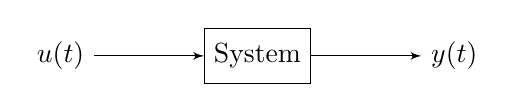
\begin{tikzpicture}[node distance=2.5cm,auto,>=latex']
	\node [input, align=center] (U) {$ u(t) $};
	\node [block, align=center] (G) [right of=U] {System};
	\node [output, align=center] (y) [right of=G] {$ y(t) $};
	\draw[->] (U) -- node {} (G);
	\draw[->] (G) -- node {} (y);
	\end{tikzpicture}
\end{center}

\exmp
\begin{center}
	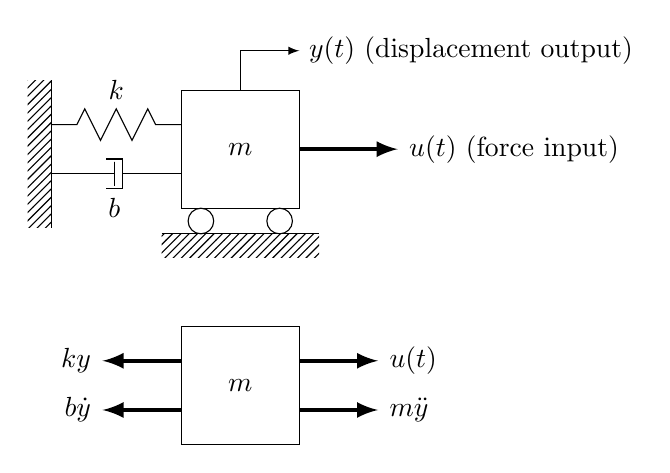
\begin{tikzpicture}
	\draw (-0.75,-0.375) rectangle node {$ m $}(0.75,1.125);
	\draw [-latex,ultra thick] (.75,0.375) -- +(1.25,0) node[right] {$ u(t) $ (force input)};
	\draw [-latex] (0,1.125) |- ++(.75,.5) node[right] {$y(t)$ (displacement output)};
	\draw[fill,pattern=north east lines,draw=none] (-2.7,-.625) rectangle (-2.4,1.25);
	\draw (-2.4,-.625) -- (-2.4,1.25);
	\draw[fill,pattern=north east lines,draw=none] (-1,-.7) rectangle (1,-1);
	\draw (-1,-.7) -- (1,-.7);
	\draw (-.5,-.5375) circle (0.1625);
	\draw (.5,-.5375) circle (0.1625);
	
	\draw (-2.4,0.6875) -- ++(0.325,0) -- ++(0.1,0.2) -- ++(0.2,-0.4) -- ++(0.2,0.4) node[above] {$ k $} -- ++(0.2,-0.4) -- ++(0.2,0.4) -- ++(0.1,-0.2) -- (-0.75,0.6875);
	\draw (-2.4,0.0625) -| ++(0.8,0.15) -- ++(0,-0.3);
	\draw (-0.75,0.0625) -| ++ (-0.75,0.1875) -- ++(-0.2,0);
	\draw (-0.75,0.0625) -| ++ (-0.75,-0.1875) -- node[below] {$ b $} ++(-0.2,0);
	
	\begin{scope}[shift={(0cm,-3cm)}]
	\draw (-0.75,-0.375) rectangle node {$ m $}(0.75,1.125);
	\draw[-latex,ultra thick] (-0.75,0.6875) -- ++(-1,0) node[left] {$ ky $};
	\draw[-latex,ultra thick] (-0.75,0.0625) -- ++(-1,0) node[left] {$ b\dot{y} $};
	\draw[-latex,ultra thick] (0.75,0.6875) -- ++(1,0) node[right] {$ u(t) $};
	\draw[-latex,ultra thick] (0.75,0.0625) -- ++(1,0) node[right] {$ m\ddot{y} $};
	\end{scope}
	
	\end{tikzpicture}
\end{center}
\[ m\ddot{y} = \sum F_x = -ky -b\dot{y}+u(t) \]
or
\[ m\ddot{y} + b\dot{y} + ky = u(t) \]
This is called the equation of motion of the system and describes the relationships between the input and output of the system. Taking the Laplace transform of both sides gives:
\[ ms^2Y + bsY + kY = U \]
Then,
\[ Y(ms^2+bs+k) = U \]
\[ \Rightarrow\quad \frac{Y}{U} = \frac{1}{ms^2+bs+k} = G(s) \]
Note that $ G(s) $ depends only on the physical parameters of the system. It does not depend on the input! That's the beauty of this:
\begin{itemize}
	\item In a sense, $ G(s) $ characterizes the system. It is a signature of the physical system. All the physics of the system (bond graphs, etc...) are tied up in $ G(s) $.
\end{itemize}
Note that
\[ G(s) = \frac{Y}{U} \quad\Rightarrow\quad Y(s) = G(s)U(s) \]
Time domain:
\begin{center}	
	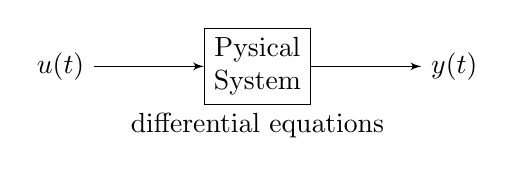
\begin{tikzpicture}[node distance=2.5cm,auto,>=latex']
	\node [input, align=center] (U) {$ u(t) $};
	\node [block, align=center] (G) [right of=U] {Pysical\\System};
	\node[below of=G,node distance=0.75cm] {differential equations};
	\node [output, align=center] (y) [right of=G] {$ y(t) $};
	\draw[->] (U) -- node {} (G);
	\draw[->] (G) -- node {} (y);
	\end{tikzpicture}
\end{center}
Laplace domain:
\begin{center}	
	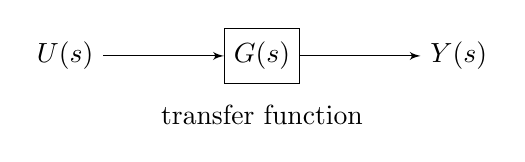
\begin{tikzpicture}[node distance=2.5cm,auto,>=latex']
	\node [input, align=center] (U) {$ U(s) $};
	\node [block, align=center] (G) [right of=U] {$ G(s) $};
	\node[below of=G,node distance=0.75cm] {transfer function};
	\node [output, align=center] (y) [right of=G] {$ Y(s) $};
	\draw[->] (U) -- node {} (G);
	\draw[->] (G) -- node {} (y);
	\end{tikzpicture}
\end{center}
\[ Y(s) = G(s)U(s) \text{ So simple!} \]

\paragraph*{Another interpretation of $ G(s) $:} Suppose that $ u(t) = \delta(t) $. Then,
\[ U(s)=1 \]
So,
\[ Y(s) = G(s)\cdot1 \]
\[ y(t) = \LT^{-1}[G(s)] \]
One nice way to think of transfer functions is as the Laplace Transform of the impulse response. This means we can measure a transfer function empirically.

\paragraph*{Transfer functions and State Space Form:} Another way to describe dynamic systems is the state-space format. The equations that relate the input to the output are converted to a set of 1st order differential equations. This can always be done for a LTI system. For a SISO system, the equations take the form
\[ \dot{\ubar{x}}(t) = \ubar{A}\ubar{x}(t) + \ubar{B}u(t) \]
\[ y(t) = \ubar{C}\ubar{x}(t)+Du(t) \]
where
\begin{itemize}
	\item $ u(t) $ is the input
	\item $ y(t) $ is the output
	\item $ x_i(t) $ are the intermediary variables, usually related to $ y(t) $ and/or its time derivatives. These are called \textbf{state variables}.
	\[ \ubar{x}(t)=\left[\begin{array}{c}
	x_1(t)\\x_2(t)\\\vdots\\x_n(t)
	\end{array}\right] \]
	is called the \textbf{state vector}.
	\item $ \ubar{A} $ is a matrix. For a SISO system, $ \ubar{B} $ and $ \ubar{C} $ are vectors and $ D $ is scalar.
\end{itemize}

\exmp
\[ m\ddot{y} + b\dot{y} + ky = u(t) \]
Let
\[ \left.\begin{array}{c} x_1=y \\ 
x_2 = \dot{y} \end{array}\right\}\ \Rightarrow\ \dot{x}_1 = x_2 \]
Then,
\[ \ddot{y}=\dot{x}_2 = \frac{1}{m}(-bx_2-kx_1+u)  \]
So,
\[ \left[\begin{array}{c}\dot{x}_1\\\dot{x}_2\end{array}\right] = \underbrace{\left[\begin{array}{c c}0 & 1\\-\dfrac{k}{m}&-\dfrac{b}{m}\end{array}\right]}_{\ubar{A}} \left[\begin{array}{c}x_1\\x_2\end{array}\right] + \underbrace{\left[\begin{array}{c}0\\\dfrac{1}{m}\end{array}\right]}_{\ubar{B}} u \]

\[ y = \underbrace{\left[\begin{array}{c c}1 & 0\end{array}\right]}_{\ubar{C}} \left[\begin{array}{c}x_1\\x_2\end{array}\right] + \underbrace{\left[\begin{array}{c}0\end{array}\right]}_{D}u \]

So, we have
\[ \dot{\ubar{x}}(t) = \ubar{A}\ubar{x}(t) + \ubar{B}u(t) \]
\[ y(t) = \ubar{C}\ubar{x}(t)+Du(t) \]

This is actually a very general way to represent LTI systems. If you are doing Bond Graphs, this is the natural outcome of your analysis. If you are using ENG102, you will naturally obtain an 2nd-order ODE that relates $ u(t) $ to $ y(t) $.

\subsection*{More general treatment}
If you have taken EME 171, you have seen that LTI systems can, in general, be represented by matrix equations of the form
\[ \underset{n\times1}{\dot{\ubar{x}}(t)} = \underset{n\times n}{\ubar{A}}\underset{n\times1}{\ubar{x}(t)} + \underset{n\times 1}{\ubar{B}}\underset{1\times1}{u(t)} \qquad \to\text{state equations} \]
\[ \underset{1\times1}{y(t)} = \underset{1\times n}{\ubar{C}}\underset{n\times1}{\ubar{x}(t)}+\underset{1\times1}{D}\underset{1\times1}{u(t)} \qquad \to\text{output equation} \]
Here, we are assuming a SISO system with $ u(t) $ as an input and $ y(t) $ as the output. This is known as the state-space representation of the system. How can we determine the transfer function of a system described in this (state-space) format? In long hand (for SISO systems) we have

\[ \underset{n\times1}{\left[\begin{array}{c} \dot{x}_1\\\dot{x}_2\\\vdots\\\dot{x}_n \end{array}\right]} = \underset{n\times n}{\left[\begin{array}{c c c c} A_{11} & A_{12} & \cdots & A_{1n} \\ A_{21} & \ddots &  &  \\ \vdots &  &  \ddots  &\vdots \\ A_{n1} &  & \cdots & A_{nn} \end{array}\right]} \underset{n\times1}{\left[\begin{array}{c} {x}_1\\{x}_2\\\vdots\\x_n \end{array}\right]} + \underset{n\times1}{\left[\begin{array}{c} B_1 \\B_2 \\\vdots\\B_n \end{array}\right]}\underset{1\times1}{u} \qquad\qquad(1) \]
\[ \underset{1\times1}{y} = \underset{1\times n}{\left[\begin{array}{c c c c} C_{1} & C_{2} & \cdots & C_{n} \end{array}\right]} \underset{n\times1}{\left[\begin{array}{c} {x}_1\\{x}_2\\\vdots\\x_n \end{array}\right]} + \underset{1\times1}{\left[\begin{array}{c} D \end{array}\right]}\underset{1\times1}{u} \qquad\qquad(2) \]

We wish to take the Laplace transform of both sides of the state and output equations. But, what does one mean by the Laplace transform of a vector or matrix?
\[ \LT\left[\begin{array}{c} {x}_1(t)\\{x}_2(t)\\\vdots\\x_n(t) \end{array}\right] \triangleq \left[\begin{array}{c} \LT[{x}_1(t)] \\ \LT[{x}_2(t)] \\ \vdots \\ \LT[x_n(t)] \end{array}\right] = \left[\begin{array}{c} X_1(s)\\X_2(s)\\\vdots\\X_n (s)\end{array}\right] \]
Now, for equation (1) above (the state equations)
\begin{align*}
\dot{x}_1 &= A_{11} x_1 + A_{12}x_2 + \ldots + A_{1n} x_n + B_1 u\\
\dot{x}_2 &= A_{21} x_1 + A_{22}x_2 + \ldots + A_{2n} x_n + B_2 u\\
&\cdots\\
\dot{x}_n &= A_{n1} x_1 + A_{n2}x_2 + \ldots + A_{nn} x_n + B_n u\\
\end{align*}
Taking the Laplace transform (assuming $ x_i(0^-)=0 $):
\begin{align*}
sX_1 &= A_{11} X_1 + A_{12}X_2 + \ldots + A_{1n} X_n + B_1 U\\
sX_2 &= A_{21} X_1 + A_{22}X_2 + \ldots + A_{2n} X_n + B_2 U\\
&\cdots\\
sX_n &= A_{n1} X_1 + A_{n2}X_2 + \ldots + A_{nn} X_n + B_n U\\
\end{align*}
Or more simply,
\[ s\ubar{X} = \ubar{A}\ubar{X} + \ubar{B}U \]
Linearity allows the process of Laplace transformation to carry over to matrices. So, we can start with 
\[ \dot{\ubar{x}}(t) = \ubar{A}\ubar{x}(t) + \ubar{B}u(t) \qquad\qquad (1)\]
\[ y(t) = \ubar{C}\ubar{x}(t)+Du(t) \qquad\qquad (2) \]
and take the Laplace transform of both sides  of (1) and (2):
\[ s\ubar{X}(s)  = \ubar{A}\ubar{X}(s)  + \ubar{B}U(s)  \qquad\qquad (3) \]
\[ Y(s)  = \ubar{C}\ubar{X}(s)  + DU(s)  \qquad\qquad (4) \]
From (3),
\[ s\ubar{X}(s) -\ubar{A}\ubar{X}(s)  =  \ubar{B}U(s)  \]
or
\[ (s\ubar{I}-\ubar{A})\ubar{X}(s)  =  \ubar{B}U(s)  \qquad\qquad (5) \]
and then
\[ \ubar{X}(s)  =  (s\ubar{I}-\ubar{A})^{-1}\ubar{B}U(s)  \qquad\qquad (6) \]
Substitute (6) into (4)
\[ Y(s)  = \ubar{C}(s\ubar{I}-\ubar{A})^{-1}\ubar{B}U(s)  + DU(s)  \]
or
\[ Y(s)  = \left(\ubar{C}(s\ubar{I}-\ubar{A})^{-1}\ubar{B}  + D\right)U(s)  \]
Hence,
\[ \Rightarrow\quad \frac{Y(s)}{U(s)} = G(s) = \underset{1\times n}{\ubar{C}}\underset{n\times n}{(s\ubar{I}-\ubar{A})^{-1}}\underset{n\times1}{\ubar{B}}  + \underset{1\times1}{D} \qquad\qquad (7)\]

One problem with (7) is that it contains a matrix inverse. Recall that for a matrix $ \ubar{M} $ that is non-singular,
\[ \ubar{M}^{-1} = \frac{\adj{\ubar{M}}}{\det{\ubar{M}}} \]
where the $ i,j $ element of $ \adj{M} $ is $ (-1)^{i+j} $ times the determinant of the matrix obtained from $ \ubar{M} $ by crossing out (removing) the $ j $-th row and $ i $-th column of $ \ubar{M} $. So, we can rewrite (7) as 
\[ G(s) = \frac{\ubar{C}\adj(s\ubar{I}-\ubar{A})\ubar{B}+D\det(s\ubar{I}-\ubar{A})}{\det(s\ubar{I}-\ubar{A})} \qquad\qquad (8)\]
This is another form of $ G(s) $.

\exmp
Example of a $ 3\times3 $ matrix inverse. Find $ \ubar{M}^{-1} $.
\[ \ubar{M}=\left[\begin{array}{c c c}
1 & 0 & 2 \\ -1 & 1 & 1 \\ 0 & 1 & -1
\end{array}\right] \]
\[ \adj(\ubar{M}) = \left[\begin{array}{c c c} 
  (-1)^{1+1}  \left|\begin{array}{c c}1&1\\1&-1\end{array}\right| & (-1)^{1+2} \left|\begin{array}{c c}0&2\\1&-1\end{array}\right| & (-1)^{1+3} \left|\begin{array}{c c}0&2\\1&1\end{array}\right| \\
  (-1)^{2+1} \left|\begin{array}{c c}-1&1\\0&-1\end{array}\right| & (-1)^{2+2} \left|\begin{array}{c c}1&2\\0&1\end{array}\right| & (-1)^{2+3} \left|\begin{array}{c c}1&2\\-1&1\end{array}\right| \\
  (-1)^{3+1}  \left|\begin{array}{c c}0&2\\1&1\end{array}\right| & (-1)^{3+2} \left|\begin{array}{c c}1&0\\0&1\end{array}\right| & (-1)^{3+3} \left|\begin{array}{c c}1&0\\-1&1\end{array}\right|
\end{array}\right] \]
\[ \adj(\ubar{M})=\left[\begin{array}{c c c}
-2 & 2 & -2 \\ -1 & -1 & -3 \\ -1 & -1 & 1
\end{array}\right] \]
\[ \det\ubar{M} = 1\cdot(1\cdot(-1)-1\cdot1) + 0\cdot(1\cdot0-(-1)\cdot(-1)) + 2\cdot((-1)\cdot1-1\cdot0) \]
\[ \det\ubar{M} = -2+0-2 = -4 \]
\[ \ubar{M}^{-1} = \frac{\adj{\ubar{M}}}{\det{\ubar{M}}} = \frac{\left[\begin{array}{c c c}
	-2 & 2 & -2 \\ -1 & -1 & -3 \\ -1 & -1 & 1
	\end{array}\right]}{-4} \]
\[ \ubar{M}^{-1} = \frac{1}{4}\left[\begin{array}{c c c}
2 & -2 & 2 \\ 1 & 1 & 3 \\ 1 & 1 & -1
\end{array}\right] \]

Returning to transfer functions: We are now in a position to determine the time-response of a system to a given input. The needed steps are:
\begin{itemize}
	\item Determine $ G(s) $ and $ U(s) $ (using given system parameters and input/output relationship to determine $ G(s) $)
	\item $ Y(s) = G(s)U(s) $
	\item $ y(t) = \LT^{-1}[G(s)U(s)] $
	\item Plot if needed.
\end{itemize}
This is easily done on a computer using Matlab software.

\exmp
\[ \ubar{A}=\left[\begin{array}{c c c} -3 & 1 & 0 \\ 0 & -6 & 1 \\ 0 & 0 & -5 \end{array}\right], \quad \ubar{B} = \left[\begin{array}{c} 0\\ 1\\ 1 \end{array}\right],\quad \ubar{C}=\left[\begin{array}{c c c} 0&1&1\end{array}\right],\quad D=0 \]
\[ s\ubar{I}-\ubar{A} = \left[\begin{array}{c c c} s+3 & -1 & 0 \\ 0 & s+6 & -1 \\ 0 & 0 & s+5 \end{array}\right] \]
\[ \adj(s\ubar{I}-\ubar{A}) = \left[\begin{array}{c c c} s^2+11s+30 & s+5 & 1 \\ 0 & s^2+8s+15 & s+3 \\ 0 & 0 & s^2+9s+18 \end{array}\right] \]
\[ \ubar{C}\adj(s\ubar{I}-\ubar{A}) = \left[\begin{array}{c c c} 0 & s^2+8s+15 & s^2+10s+21\end{array}\right] \]
\[ \ubar{C}\adj(s\ubar{I}-\ubar{A})\ubar{B} = 2s^2+18s+36 = 2(s+3)(s+6) \]
\[ \det(s\ubar{I}-\ubar{A}) = (s+3)(s+6)(s+5)\]
Hence,
\[ G(s) = \frac{2\cancel{(s+3)}\cancel{(s+6)}}{\cancel{(s+3)}\cancel{(s+6)}(s+5)} = \frac{2}{s+5} \]
	

Let's say that the input is a step function $ u(t)=1 $, so then $ U(s)=1/s $. Then
\[ Y(s) = G(s)U(s) = \frac{2}{s(s+5)} = \frac{R_1}{s}+\frac{R_2}{s+5} \]
where
\[ R_1=sY(s)\Big|_{s=0} = \frac{2}{5},\quad R_2=(s+5)Y(s)\Big|_{s=-5} = -\frac{2}{5} \]
So,
\[ Y(s) = \frac{2}{5s}-\frac{2}{5(s+5)} \]
\[ y(t) = \left(\frac{2}{5} -\frac{2}{5}e^{-5t}   \right) 1(t) \]

\section*{State-Space Continued}
If $ \ubar{A} $ is an $ n\times n $ matrix, then $ \det(sI-{\ubar{A}}) $ is a polynomial of order $ n $, each element of $ \adj(sI-{\ubar{A}}) $ is a polynomial of order $ <n $. Therefore,
\[ \ubar{C}(s\ubar{I}-\ubar{A})^{-1}\ubar{B}\]
is a polynomial of order (degree) $ <n $. So, if $ D=0 $ then $ G(s) $ is strictly proper. If $ D\neq0 $, then $ G(s) $ is proper. $ G(s) $ can never be improper!

\subsection*{Poles and zeros in state space}
To obtain the poles of $ G(s) $, set the denominator of $ G(s) $ to zero and solve for $ s $. That is,
\[ \text{solve for }s:\quad \det(sI-A)=0 \]
Poles depend on the $ \ubar{A} $ matrix only! $ \ubar{B} $, $ \ubar{C} $, and $ D $ have no effect on the poles. To get the zeros of $ G(s) $, solve
\[ \ubar{C}\adj(s\ubar{I}-\ubar{A})\ubar{B}+D\det(s\ubar{I}-\ubar{A}) = 0 \]
for $ s $. So, the zeros depend on $ \ubar{A} $, $ \ubar{B} $, $ \ubar{C} $, and $ D $.











\end{document}

